\documentclass[1p]{elsarticle_modified}
%\bibliographystyle{elsarticle-num}

%\usepackage[colorlinks]{hyperref}
%\usepackage{abbrmath_seonhwa} %\Abb, \Ascr, \Acal ,\Abf, \Afrak
\usepackage{amsfonts}
\usepackage{amssymb}
\usepackage{amsmath}
\usepackage{amsthm}
\usepackage{scalefnt}
\usepackage{amsbsy}
\usepackage{kotex}
\usepackage{caption}
\usepackage{subfig}
\usepackage{color}
\usepackage{graphicx}
\usepackage{xcolor} %% white, black, red, green, blue, cyan, magenta, yellow
\usepackage{float}
\usepackage{setspace}
\usepackage{hyperref}

\usepackage{tikz}
\usetikzlibrary{arrows}

\usepackage{multirow}
\usepackage{array} % fixed length table
\usepackage{hhline}

%%%%%%%%%%%%%%%%%%%%%
\makeatletter
\renewcommand*\env@matrix[1][\arraystretch]{%
	\edef\arraystretch{#1}%
	\hskip -\arraycolsep
	\let\@ifnextchar\new@ifnextchar
	\array{*\c@MaxMatrixCols c}}
\makeatother %https://tex.stackexchange.com/questions/14071/how-can-i-increase-the-line-spacing-in-a-matrix
%%%%%%%%%%%%%%%

\usepackage[normalem]{ulem}

\newcommand{\msout}[1]{\ifmmode\text{\sout{\ensuremath{#1}}}\else\sout{#1}\fi}
%SOURCE: \msout is \stkout macro in https://tex.stackexchange.com/questions/20609/strikeout-in-math-mode

\newcommand{\cancel}[1]{
	\ifmmode
	{\color{red}\msout{#1}}
	\else
	{\color{red}\sout{#1}}
	\fi
}

\newcommand{\add}[1]{
	{\color{blue}\uwave{#1}}
}

\newcommand{\replace}[2]{
	\ifmmode
	{\color{red}\msout{#1}}{\color{blue}\uwave{#2}}
	\else
	{\color{red}\sout{#1}}{\color{blue}\uwave{#2}}
	\fi
}

\newcommand{\Sol}{\mathcal{S}} %segment
\newcommand{\D}{D} %diagram
\newcommand{\A}{\mathcal{A}} %arc


%%%%%%%%%%%%%%%%%%%%%%%%%%%%%5 test

\def\sl{\operatorname{\textup{SL}}(2,\Cbb)}
\def\psl{\operatorname{\textup{PSL}}(2,\Cbb)}
\def\quan{\mkern 1mu \triangleright \mkern 1mu}

\theoremstyle{definition}
\newtheorem{thm}{Theorem}[section]
\newtheorem{prop}[thm]{Proposition}
\newtheorem{lem}[thm]{Lemma}
\newtheorem{ques}[thm]{Question}
\newtheorem{cor}[thm]{Corollary}
\newtheorem{defn}[thm]{Definition}
\newtheorem{exam}[thm]{Example}
\newtheorem{rmk}[thm]{Remark}
\newtheorem{alg}[thm]{Algorithm}

\newcommand{\I}{\sqrt{-1}}
\begin{document}

%\begin{frontmatter}
%
%\title{Boundary parabolic representations of knots up to 8 crossings}
%
%%% Group authors per affiliation:
%\author{Yunhi Cho} 
%\address{Department of Mathematics, University of Seoul, Seoul, Korea}
%\ead{yhcho@uos.ac.kr}
%
%
%\author{Seonhwa Kim} %\fnref{s_kim}}
%\address{Center for Geometry and Physics, Institute for Basic Science, Pohang, 37673, Korea}
%\ead{ryeona17@ibs.re.kr}
%
%\author{Hyuk Kim}
%\address{Department of Mathematical Sciences, Seoul National University, Seoul 08826, Korea}
%\ead{hyukkim@snu.ac.kr}
%
%\author{Seokbeom Yoon}
%\address{Department of Mathematical Sciences, Seoul National University, Seoul, 08826,  Korea}
%\ead{sbyoon15@snu.ac.kr}
%
%\begin{abstract}
%We find all boundary parabolic representation of knots up to 8 crossings.
%
%\end{abstract}
%\begin{keyword}
%    \MSC[2010] 57M25 
%\end{keyword}
%
%\end{frontmatter}

%\linenumbers
%\tableofcontents
%
\newcommand\colored[1]{\textcolor{white}{\rule[-0.35ex]{0.8em}{1.4ex}}\kern-0.8em\color{red} #1}%
%\newcommand\colored[1]{\textcolor{white}{ #1}\kern-2.17ex	\textcolor{white}{ #1}\kern-1.81ex	\textcolor{white}{ #1}\kern-2.15ex\color{red}#1	}

{\Large $\underline{12a_{0293}~(K12a_{0293})}$}

\setlength{\tabcolsep}{10pt}
\renewcommand{\arraystretch}{1.6}
\vspace{1cm}\begin{tabular}{m{100pt}>{\centering\arraybackslash}m{274pt}}
\multirow{5}{120pt}{
	\centering
	\includegraphics[width=112pt]{../../../GIT/diagram.site/Diagrams/png/1094_12a_0293.png}\\
\ \ \ A knot diagram\footnotemark}&
\allowdisplaybreaks
\textbf{Linearized knot diagam} \\
\cline{2-2}
 &
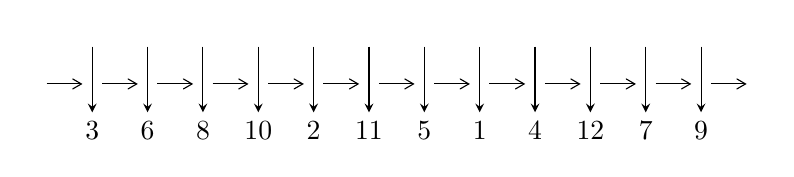
\begin{tikzpicture}[x=20pt, y=17pt]
	% nodes
	\node (C0) at (0, 0) {};
	\node (C1) at (1, 0) {};
	\node (C1U) at (1, +1) {};
	\node (C1D) at (1, -1) {3};

	\node (C2) at (2, 0) {};
	\node (C2U) at (2, +1) {};
	\node (C2D) at (2, -1) {6};

	\node (C3) at (3, 0) {};
	\node (C3U) at (3, +1) {};
	\node (C3D) at (3, -1) {8};

	\node (C4) at (4, 0) {};
	\node (C4U) at (4, +1) {};
	\node (C4D) at (4, -1) {10};

	\node (C5) at (5, 0) {};
	\node (C5U) at (5, +1) {};
	\node (C5D) at (5, -1) {2};

	\node (C6) at (6, 0) {};
	\node (C6U) at (6, +1) {};
	\node (C6D) at (6, -1) {11};

	\node (C7) at (7, 0) {};
	\node (C7U) at (7, +1) {};
	\node (C7D) at (7, -1) {5};

	\node (C8) at (8, 0) {};
	\node (C8U) at (8, +1) {};
	\node (C8D) at (8, -1) {1};

	\node (C9) at (9, 0) {};
	\node (C9U) at (9, +1) {};
	\node (C9D) at (9, -1) {4};

	\node (C10) at (10, 0) {};
	\node (C10U) at (10, +1) {};
	\node (C10D) at (10, -1) {12};

	\node (C11) at (11, 0) {};
	\node (C11U) at (11, +1) {};
	\node (C11D) at (11, -1) {7};

	\node (C12) at (12, 0) {};
	\node (C12U) at (12, +1) {};
	\node (C12D) at (12, -1) {9};
	\node (C13) at (13, 0) {};

	% arrows
	\draw[->,>={angle 60}]
	(C0) edge (C1) (C1) edge (C2) (C2) edge (C3) (C3) edge (C4) (C4) edge (C5) (C5) edge (C6) (C6) edge (C7) (C7) edge (C8) (C8) edge (C9) (C9) edge (C10) (C10) edge (C11) (C11) edge (C12) (C12) edge (C13) ;	\draw[->,>=stealth]
	(C1U) edge (C1D) (C2U) edge (C2D) (C3U) edge (C3D) (C4U) edge (C4D) (C5U) edge (C5D) (C6U) edge (C6D) (C7U) edge (C7D) (C8U) edge (C8D) (C9U) edge (C9D) (C10U) edge (C10D) (C11U) edge (C11D) (C12U) edge (C12D) ;
	\end{tikzpicture} \\
\hhline{~~} \\& 
\textbf{Solving Sequence} \\ \cline{2-2} 
 &
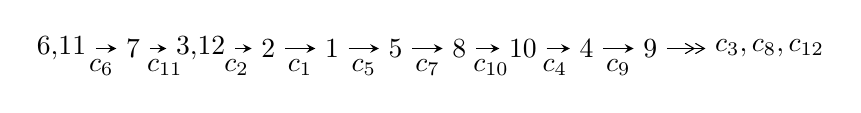
\begin{tikzpicture}[x=23pt, y=7pt]
	% node
	\node (A0) at (-1/8, 0) {6,11};
	\node (A1) at (1, 0) {7};
	\node (A2) at (33/16, 0) {3,12};
	\node (A3) at (25/8, 0) {2};
	\node (A4) at (33/8, 0) {1};
	\node (A5) at (41/8, 0) {5};
	\node (A6) at (49/8, 0) {8};
	\node (A7) at (57/8, 0) {10};
	\node (A8) at (65/8, 0) {4};
	\node (A9) at (73/8, 0) {9};
	\node (C1) at (1/2, -1) {$c_{6}$};
	\node (C2) at (3/2, -1) {$c_{11}$};
	\node (C3) at (21/8, -1) {$c_{2}$};
	\node (C4) at (29/8, -1) {$c_{1}$};
	\node (C5) at (37/8, -1) {$c_{5}$};
	\node (C6) at (45/8, -1) {$c_{7}$};
	\node (C7) at (53/8, -1) {$c_{10}$};
	\node (C8) at (61/8, -1) {$c_{4}$};
	\node (C9) at (69/8, -1) {$c_{9}$};
	\node (A10) at (11, 0) {$c_{3},c_{8},c_{12}$};

	% edge
	\draw[->,>=stealth]	
	(A0) edge (A1) (A1) edge (A2) (A2) edge (A3) (A3) edge (A4) (A4) edge (A5) (A5) edge (A6) (A6) edge (A7) (A7) edge (A8) (A8) edge (A9) ;
	\draw[->>,>={angle 60}]	
	(A9) edge (A10);
\end{tikzpicture} \\ 

\end{tabular} \\

\footnotetext{
The image of knot diagram is generated by the software ``\textbf{Draw programme}" developed by Andrew Bartholomew(\url{http://www.layer8.co.uk/maths/draw/index.htm\#Running-draw}), where we modified some parts for our purpose(\url{https://github.com/CATsTAILs/LinksPainter}).
}\phantom \\ \newline 
\centering \textbf{Ideals for irreducible components\footnotemark of $X_{\text{par}}$} 
 
\begin{align*}
I^u_{1}&=\langle 
-2.68620\times10^{394} u^{141}+2.89813\times10^{395} u^{140}+\cdots+1.40096\times10^{396} b-3.85850\times10^{398},\\
\phantom{I^u_{1}}&\phantom{= \langle  }-2.69292\times10^{397} u^{141}-7.48767\times10^{397} u^{140}+\cdots+8.29864\times10^{397} a+9.29056\times10^{400},\\
\phantom{I^u_{1}}&\phantom{= \langle  }u^{142}+2 u^{141}+\cdots+547 u-1007\rangle \\
I^u_{2}&=\langle 
11 u^{28}+2 u^{27}+\cdots+b+1,\;36 u^{28}-17 u^{27}+\cdots+a+57,\;u^{29}- u^{28}+\cdots+4 u-1\rangle \\
\\
\end{align*}
\raggedright * 2 irreducible components of $\dim_{\mathbb{C}}=0$, with total 171 representations.\\
\footnotetext{All coefficients of polynomials are rational numbers. But the coefficients are sometimes approximated in decimal forms when there is not enough margin.}
\newpage
\renewcommand{\arraystretch}{1}
\centering \section*{I. $I^u_{1}= \langle -2.69\times10^{394} u^{141}+2.90\times10^{395} u^{140}+\cdots+1.40\times10^{396} b-3.86\times10^{398},\;-2.69\times10^{397} u^{141}-7.49\times10^{397} u^{140}+\cdots+8.30\times10^{397} a+9.29\times10^{400},\;u^{142}+2 u^{141}+\cdots+547 u-1007 \rangle$}
\flushleft \textbf{(i) Arc colorings}\\
\begin{tabular}{m{7pt} m{180pt} m{7pt} m{180pt} }
\flushright $a_{6}=$&$\begin{pmatrix}1\\0\end{pmatrix}$ \\
\flushright $a_{11}=$&$\begin{pmatrix}0\\u\end{pmatrix}$ \\
\flushright $a_{7}=$&$\begin{pmatrix}1\\u^2\end{pmatrix}$ \\
\flushright $a_{3}=$&$\begin{pmatrix}0.324502 u^{141}+0.902277 u^{140}+\cdots+2024.09 u-1119.53\\0.0191740 u^{141}-0.206867 u^{140}+\cdots-570.651 u+275.418\end{pmatrix}$ \\
\flushright $a_{12}=$&$\begin{pmatrix}- u\\- u^3+u\end{pmatrix}$ \\
\flushright $a_{2}=$&$\begin{pmatrix}0.343676 u^{141}+0.695410 u^{140}+\cdots+1453.44 u-844.109\\0.0191740 u^{141}-0.206867 u^{140}+\cdots-570.651 u+275.418\end{pmatrix}$ \\
\flushright $a_{1}=$&$\begin{pmatrix}0.445228 u^{141}+0.992377 u^{140}+\cdots+1813.92 u-1079.17\\-1.24464 u^{141}-1.82063 u^{140}+\cdots-2017.86 u+1441.73\end{pmatrix}$ \\
\flushright $a_{5}=$&$\begin{pmatrix}-0.454052 u^{141}-0.769538 u^{140}+\cdots-1265.24 u+766.555\\-1.22762 u^{141}-1.01892 u^{140}+\cdots+23.3711 u+500.852\end{pmatrix}$ \\
\flushright $a_{8}=$&$\begin{pmatrix}-0.723879 u^{141}-0.854490 u^{140}+\cdots+584.319 u-16.5073\\0.555025 u^{141}+0.280459 u^{140}+\cdots-836.186 u+46.1797\end{pmatrix}$ \\
\flushright $a_{10}=$&$\begin{pmatrix}u^3\\u^5- u^3+u\end{pmatrix}$ \\
\flushright $a_{4}=$&$\begin{pmatrix}0.235017 u^{141}-0.253990 u^{140}+\cdots-1520.59 u+620.267\\-1.37505 u^{141}-1.24854 u^{140}+\cdots-244.129 u+679.355\end{pmatrix}$ \\
\flushright $a_{9}=$&$\begin{pmatrix}-1.62936 u^{141}-1.75855 u^{140}+\cdots-1055.05 u+1207.03\\0.550954 u^{141}+0.242025 u^{140}+\cdots-673.973 u+8.66774\end{pmatrix}$\\&\end{tabular}
\flushleft \textbf{(ii) Obstruction class $= -1$}\\~\\
\flushleft \textbf{(iii) Cusp Shapes $= 0.391067 u^{141}-0.798487 u^{140}+\cdots-3673.90 u+1241.22$}\\~\\
\newpage\renewcommand{\arraystretch}{1}
\flushleft \textbf{(iv) u-Polynomials at the component}\newline \\
\begin{tabular}{m{50pt}|m{274pt}}
Crossings & \hspace{64pt}u-Polynomials at each crossing \\
\hline $$\begin{aligned}c_{1}\end{aligned}$$&$\begin{aligned}
&u^{142}+54 u^{141}+\cdots+370442 u+6241
\end{aligned}$\\
\hline $$\begin{aligned}c_{2},c_{5}\end{aligned}$$&$\begin{aligned}
&u^{142}+8 u^{141}+\cdots-566 u-79
\end{aligned}$\\
\hline $$\begin{aligned}c_{3}\end{aligned}$$&$\begin{aligned}
&u^{142}+u^{141}+\cdots+16848 u-905
\end{aligned}$\\
\hline $$\begin{aligned}c_{4},c_{9}\end{aligned}$$&$\begin{aligned}
&u^{142}- u^{141}+\cdots+10 u^2-1
\end{aligned}$\\
\hline $$\begin{aligned}c_{6},c_{11}\end{aligned}$$&$\begin{aligned}
&u^{142}-2 u^{141}+\cdots-547 u-1007
\end{aligned}$\\
\hline $$\begin{aligned}c_{7}\end{aligned}$$&$\begin{aligned}
&u^{142}-3 u^{141}+\cdots-8672 u+4937
\end{aligned}$\\
\hline $$\begin{aligned}c_{8},c_{12}\end{aligned}$$&$\begin{aligned}
&u^{142}-4 u^{141}+\cdots+11237 u+289
\end{aligned}$\\
\hline $$\begin{aligned}c_{10}\end{aligned}$$&$\begin{aligned}
&u^{142}+58 u^{141}+\cdots+38359781 u+1014049
\end{aligned}$\\
\hline
\end{tabular}\\~\\
\newpage\renewcommand{\arraystretch}{1}
\flushleft \textbf{(v) Riley Polynomials at the component}\newline \\
\begin{tabular}{m{50pt}|m{274pt}}
Crossings & \hspace{64pt}Riley Polynomials at each crossing \\
\hline $$\begin{aligned}c_{1}\end{aligned}$$&$\begin{aligned}
&y^{142}+82 y^{141}+\cdots-5472163826 y+38950081
\end{aligned}$\\
\hline $$\begin{aligned}c_{2},c_{5}\end{aligned}$$&$\begin{aligned}
&y^{142}-54 y^{141}+\cdots-370442 y+6241
\end{aligned}$\\
\hline $$\begin{aligned}c_{3}\end{aligned}$$&$\begin{aligned}
&y^{142}+27 y^{141}+\cdots-80000234 y+819025
\end{aligned}$\\
\hline $$\begin{aligned}c_{4},c_{9}\end{aligned}$$&$\begin{aligned}
&y^{142}-89 y^{141}+\cdots-20 y+1
\end{aligned}$\\
\hline $$\begin{aligned}c_{6},c_{11}\end{aligned}$$&$\begin{aligned}
&y^{142}-58 y^{141}+\cdots-38359781 y+1014049
\end{aligned}$\\
\hline $$\begin{aligned}c_{7}\end{aligned}$$&$\begin{aligned}
&y^{142}+15 y^{141}+\cdots+1536104854 y+24373969
\end{aligned}$\\
\hline $$\begin{aligned}c_{8},c_{12}\end{aligned}$$&$\begin{aligned}
&y^{142}+104 y^{141}+\cdots-98905915 y+83521
\end{aligned}$\\
\hline $$\begin{aligned}c_{10}\end{aligned}$$&$\begin{aligned}
&y^{142}+66 y^{141}+\cdots+28207829072127 y+1028295374401
\end{aligned}$\\
\hline
\end{tabular}\\~\\
\newpage\flushleft \textbf{(vi) Complex Volumes and Cusp Shapes}
$$\begin{array}{c|c|c}  
\text{Solutions to }I^u_{1}& \I (\text{vol} + \sqrt{-1}CS) & \text{Cusp shape}\\
 \hline 
\begin{aligned}
u &= \phantom{-}0.852421 + 0.522282 I \\
a &= \phantom{-}1.74806 - 3.40367 I \\
b &= \phantom{-}0.859735 + 0.616722 I\end{aligned}
 & \phantom{-}2.99761 - 1.03355 I & \phantom{-0.000000 } 0 \\ \hline\begin{aligned}
u &= \phantom{-}0.852421 - 0.522282 I \\
a &= \phantom{-}1.74806 + 3.40367 I \\
b &= \phantom{-}0.859735 - 0.616722 I\end{aligned}
 & \phantom{-}2.99761 + 1.03355 I & \phantom{-0.000000 } 0 \\ \hline\begin{aligned}
u &= -0.928961 + 0.343247 I \\
a &= -1.079520 - 0.573628 I \\
b &= -1.182340 - 0.121222 I\end{aligned}
 & -3.19866 + 1.20959 I & \phantom{-0.000000 } 0 \\ \hline\begin{aligned}
u &= -0.928961 - 0.343247 I \\
a &= -1.079520 + 0.573628 I \\
b &= -1.182340 + 0.121222 I\end{aligned}
 & -3.19866 - 1.20959 I & \phantom{-0.000000 } 0 \\ \hline\begin{aligned}
u &= \phantom{-}0.869382 + 0.524205 I \\
a &= -1.01437 + 2.22245 I \\
b &= \phantom{-}0.835100 - 0.706450 I\end{aligned}
 & \phantom{-}2.93974 - 3.19163 I & \phantom{-0.000000 } 0 \\ \hline\begin{aligned}
u &= \phantom{-}0.869382 - 0.524205 I \\
a &= -1.01437 - 2.22245 I \\
b &= \phantom{-}0.835100 + 0.706450 I\end{aligned}
 & \phantom{-}2.93974 + 3.19163 I & \phantom{-0.000000 } 0 \\ \hline\begin{aligned}
u &= \phantom{-}0.672295 + 0.763385 I \\
a &= -0.16994 - 1.79953 I \\
b &= \phantom{-}0.647232 + 0.959592 I\end{aligned}
 & \phantom{-}8.07878 + 0.85121 I & \phantom{-0.000000 } 0 \\ \hline\begin{aligned}
u &= \phantom{-}0.672295 - 0.763385 I \\
a &= -0.16994 + 1.79953 I \\
b &= \phantom{-}0.647232 - 0.959592 I\end{aligned}
 & \phantom{-}8.07878 - 0.85121 I & \phantom{-0.000000 } 0 \\ \hline\begin{aligned}
u &= \phantom{-}0.816739 + 0.607186 I \\
a &= -2.34879 - 0.13672 I \\
b &= \phantom{-}0.850895 - 0.622594 I\end{aligned}
 & \phantom{-}3.02412 + 3.83131 I & \phantom{-0.000000 } 0 \\ \hline\begin{aligned}
u &= \phantom{-}0.816739 - 0.607186 I \\
a &= -2.34879 + 0.13672 I \\
b &= \phantom{-}0.850895 + 0.622594 I\end{aligned}
 & \phantom{-}3.02412 - 3.83131 I & \phantom{-0.000000 } 0\\
 \hline 
 \end{array}$$\newpage$$\begin{array}{c|c|c}  
\text{Solutions to }I^u_{1}& \I (\text{vol} + \sqrt{-1}CS) & \text{Cusp shape}\\
 \hline 
\begin{aligned}
u &= \phantom{-}0.886616 + 0.422301 I \\
a &= \phantom{-}0.286300 + 0.129508 I \\
b &= -1.131980 + 0.715887 I\end{aligned}
 & -1.56995 + 1.18711 I & \phantom{-0.000000 } 0 \\ \hline\begin{aligned}
u &= \phantom{-}0.886616 - 0.422301 I \\
a &= \phantom{-}0.286300 - 0.129508 I \\
b &= -1.131980 - 0.715887 I\end{aligned}
 & -1.56995 - 1.18711 I & \phantom{-0.000000 } 0 \\ \hline\begin{aligned}
u &= -0.953198 + 0.370460 I \\
a &= -0.445465 - 0.726537 I \\
b &= -1.40087 - 0.19638 I\end{aligned}
 & -3.10094 + 1.36359 I & \phantom{-0.000000 } 0 \\ \hline\begin{aligned}
u &= -0.953198 - 0.370460 I \\
a &= -0.445465 + 0.726537 I \\
b &= -1.40087 + 0.19638 I\end{aligned}
 & -3.10094 - 1.36359 I & \phantom{-0.000000 } 0 \\ \hline\begin{aligned}
u &= \phantom{-}0.618279 + 0.818936 I \\
a &= -0.82090 + 1.24911 I \\
b &= \phantom{-}1.079850 - 0.753387 I\end{aligned}
 & \phantom{-}6.71061 + 7.10649 I & \phantom{-0.000000 } 0 \\ \hline\begin{aligned}
u &= \phantom{-}0.618279 - 0.818936 I \\
a &= -0.82090 - 1.24911 I \\
b &= \phantom{-}1.079850 + 0.753387 I\end{aligned}
 & \phantom{-}6.71061 - 7.10649 I & \phantom{-0.000000 } 0 \\ \hline\begin{aligned}
u &= \phantom{-}0.509160 + 0.822000 I \\
a &= \phantom{-}0.27897 - 1.61555 I \\
b &= -1.010670 + 0.646060 I\end{aligned}
 & -0.76963 + 6.91366 I & \phantom{-0.000000 } 0 \\ \hline\begin{aligned}
u &= \phantom{-}0.509160 - 0.822000 I \\
a &= \phantom{-}0.27897 + 1.61555 I \\
b &= -1.010670 - 0.646060 I\end{aligned}
 & -0.76963 - 6.91366 I & \phantom{-0.000000 } 0 \\ \hline\begin{aligned}
u &= -0.826303 + 0.500457 I \\
a &= \phantom{-}1.49305 + 0.62863 I \\
b &= -1.000330 - 0.949949 I\end{aligned}
 & -0.81298 - 1.57306 I & \phantom{-0.000000 } 0 \\ \hline\begin{aligned}
u &= -0.826303 - 0.500457 I \\
a &= \phantom{-}1.49305 - 0.62863 I \\
b &= -1.000330 + 0.949949 I\end{aligned}
 & -0.81298 + 1.57306 I & \phantom{-0.000000 } 0\\
 \hline 
 \end{array}$$\newpage$$\begin{array}{c|c|c}  
\text{Solutions to }I^u_{1}& \I (\text{vol} + \sqrt{-1}CS) & \text{Cusp shape}\\
 \hline 
\begin{aligned}
u &= \phantom{-}0.930284 + 0.254180 I \\
a &= \phantom{-}0.998616 - 0.488365 I \\
b &= -0.664075 + 0.912474 I\end{aligned}
 & -0.38593 + 1.76929 I & \phantom{-0.000000 } 0 \\ \hline\begin{aligned}
u &= \phantom{-}0.930284 - 0.254180 I \\
a &= \phantom{-}0.998616 + 0.488365 I \\
b &= -0.664075 - 0.912474 I\end{aligned}
 & -0.38593 - 1.76929 I & \phantom{-0.000000 } 0 \\ \hline\begin{aligned}
u &= -0.898633 + 0.516167 I \\
a &= -0.60340 - 2.44721 I \\
b &= -1.08826 + 0.92073 I\end{aligned}
 & -1.06998 + 5.69980 I & \phantom{-0.000000 } 0 \\ \hline\begin{aligned}
u &= -0.898633 - 0.516167 I \\
a &= -0.60340 + 2.44721 I \\
b &= -1.08826 - 0.92073 I\end{aligned}
 & -1.06998 - 5.69980 I & \phantom{-0.000000 } 0 \\ \hline\begin{aligned}
u &= \phantom{-}0.560948 + 0.779853 I \\
a &= \phantom{-}0.731956 + 1.195910 I \\
b &= -0.595659 - 0.690517 I\end{aligned}
 & \phantom{-}0.43167 + 1.73263 I & \phantom{-0.000000 } 0 \\ \hline\begin{aligned}
u &= \phantom{-}0.560948 - 0.779853 I \\
a &= \phantom{-}0.731956 - 1.195910 I \\
b &= -0.595659 + 0.690517 I\end{aligned}
 & \phantom{-}0.43167 - 1.73263 I & \phantom{-0.000000 } 0 \\ \hline\begin{aligned}
u &= \phantom{-}1.033110 + 0.123064 I \\
a &= \phantom{-}1.059870 - 0.179354 I \\
b &= \phantom{-}0.922437 - 0.459297 I\end{aligned}
 & -2.24178 + 1.78905 I & \phantom{-0.000000 } 0 \\ \hline\begin{aligned}
u &= \phantom{-}1.033110 - 0.123064 I \\
a &= \phantom{-}1.059870 + 0.179354 I \\
b &= \phantom{-}0.922437 + 0.459297 I\end{aligned}
 & -2.24178 - 1.78905 I & \phantom{-0.000000 } 0 \\ \hline\begin{aligned}
u &= -0.831311 + 0.460358 I \\
a &= -0.664289 + 0.801812 I \\
b &= \phantom{-}0.652636 - 0.765992 I\end{aligned}
 & \phantom{-}2.51745 + 0.76617 I & \phantom{-0.000000 } 0 \\ \hline\begin{aligned}
u &= -0.831311 - 0.460358 I \\
a &= -0.664289 - 0.801812 I \\
b &= \phantom{-}0.652636 + 0.765992 I\end{aligned}
 & \phantom{-}2.51745 - 0.76617 I & \phantom{-0.000000 } 0\\
 \hline 
 \end{array}$$\newpage$$\begin{array}{c|c|c}  
\text{Solutions to }I^u_{1}& \I (\text{vol} + \sqrt{-1}CS) & \text{Cusp shape}\\
 \hline 
\begin{aligned}
u &= \phantom{-}0.862941 + 0.602584 I \\
a &= -0.23863 + 1.41189 I \\
b &= -0.693700 - 0.779435 I\end{aligned}
 & -0.40441 - 4.89013 I & \phantom{-0.000000 } 0 \\ \hline\begin{aligned}
u &= \phantom{-}0.862941 - 0.602584 I \\
a &= -0.23863 - 1.41189 I \\
b &= -0.693700 + 0.779435 I\end{aligned}
 & -0.40441 + 4.89013 I & \phantom{-0.000000 } 0 \\ \hline\begin{aligned}
u &= \phantom{-}0.725636 + 0.591320 I \\
a &= \phantom{-}0.871670 - 0.629506 I \\
b &= -0.459795 + 0.602011 I\end{aligned}
 & -0.0147121 + 0.0682797 I & \phantom{-0.000000 } 0 \\ \hline\begin{aligned}
u &= \phantom{-}0.725636 - 0.591320 I \\
a &= \phantom{-}0.871670 + 0.629506 I \\
b &= -0.459795 - 0.602011 I\end{aligned}
 & -0.0147121 - 0.0682797 I & \phantom{-0.000000 } 0 \\ \hline\begin{aligned}
u &= \phantom{-}0.887664 + 0.589588 I \\
a &= -1.20735 - 2.14295 I \\
b &= \phantom{-}0.879629 + 0.692664 I\end{aligned}
 & \phantom{-}2.80012 - 8.55528 I & \phantom{-0.000000 } 0 \\ \hline\begin{aligned}
u &= \phantom{-}0.887664 - 0.589588 I \\
a &= -1.20735 + 2.14295 I \\
b &= \phantom{-}0.879629 - 0.692664 I\end{aligned}
 & \phantom{-}2.80012 + 8.55528 I & \phantom{-0.000000 } 0 \\ \hline\begin{aligned}
u &= -0.516624 + 0.940358 I \\
a &= \phantom{-}0.40988 - 1.61323 I \\
b &= -0.613362 + 0.891946 I\end{aligned}
 & \phantom{-}5.24057 - 7.32404 I & \phantom{-0.000000 } 0 \\ \hline\begin{aligned}
u &= -0.516624 - 0.940358 I \\
a &= \phantom{-}0.40988 + 1.61323 I \\
b &= -0.613362 - 0.891946 I\end{aligned}
 & \phantom{-}5.24057 + 7.32404 I & \phantom{-0.000000 } 0 \\ \hline\begin{aligned}
u &= \phantom{-}0.569659 + 0.727782 I \\
a &= \phantom{-}0.968075 - 0.287809 I \\
b &= -0.713803 - 0.051834 I\end{aligned}
 & \phantom{-}0.598697 + 0.714553 I & \phantom{-0.000000 } 0 \\ \hline\begin{aligned}
u &= \phantom{-}0.569659 - 0.727782 I \\
a &= \phantom{-}0.968075 + 0.287809 I \\
b &= -0.713803 + 0.051834 I\end{aligned}
 & \phantom{-}0.598697 - 0.714553 I & \phantom{-0.000000 } 0\\
 \hline 
 \end{array}$$\newpage$$\begin{array}{c|c|c}  
\text{Solutions to }I^u_{1}& \I (\text{vol} + \sqrt{-1}CS) & \text{Cusp shape}\\
 \hline 
\begin{aligned}
u &= \phantom{-}0.115177 + 1.072180 I \\
a &= -0.123782 + 1.343500 I \\
b &= \phantom{-}0.752483 - 0.668716 I\end{aligned}
 & \phantom{-}4.75781 + 2.09794 I & \phantom{-0.000000 } 0 \\ \hline\begin{aligned}
u &= \phantom{-}0.115177 - 1.072180 I \\
a &= -0.123782 - 1.343500 I \\
b &= \phantom{-}0.752483 + 0.668716 I\end{aligned}
 & \phantom{-}4.75781 - 2.09794 I & \phantom{-0.000000 } 0 \\ \hline\begin{aligned}
u &= -0.741271 + 0.533819 I \\
a &= \phantom{-}1.08179 + 0.96471 I \\
b &= \phantom{-}0.554539 + 0.273850 I\end{aligned}
 & \phantom{-}2.62137 + 2.52187 I & \phantom{-0.000000 } 0 \\ \hline\begin{aligned}
u &= -0.741271 - 0.533819 I \\
a &= \phantom{-}1.08179 - 0.96471 I \\
b &= \phantom{-}0.554539 - 0.273850 I\end{aligned}
 & \phantom{-}2.62137 - 2.52187 I & \phantom{-0.000000 } 0 \\ \hline\begin{aligned}
u &= -1.066580 + 0.218214 I \\
a &= \phantom{-}1.70743 + 1.44159 I \\
b &= \phantom{-}1.003330 - 0.194292 I\end{aligned}
 & -8.84637 + 0.96973 I & \phantom{-0.000000 } 0 \\ \hline\begin{aligned}
u &= -1.066580 - 0.218214 I \\
a &= \phantom{-}1.70743 - 1.44159 I \\
b &= \phantom{-}1.003330 + 0.194292 I\end{aligned}
 & -8.84637 - 0.96973 I & \phantom{-0.000000 } 0 \\ \hline\begin{aligned}
u &= \phantom{-}0.984927 + 0.486064 I \\
a &= -0.65608 + 1.72958 I \\
b &= -1.197500 - 0.431898 I\end{aligned}
 & -2.16249 - 4.43464 I & \phantom{-0.000000 } 0 \\ \hline\begin{aligned}
u &= \phantom{-}0.984927 - 0.486064 I \\
a &= -0.65608 - 1.72958 I \\
b &= -1.197500 + 0.431898 I\end{aligned}
 & -2.16249 + 4.43464 I & \phantom{-0.000000 } 0 \\ \hline\begin{aligned}
u &= -0.894072 + 0.087314 I \\
a &= \phantom{-}1.58003 + 0.02822 I \\
b &= \phantom{-}1.071510 - 0.596786 I\end{aligned}
 & \phantom{-}0.65212 + 7.13519 I & \phantom{-0.000000 } 0 \\ \hline\begin{aligned}
u &= -0.894072 - 0.087314 I \\
a &= \phantom{-}1.58003 - 0.02822 I \\
b &= \phantom{-}1.071510 + 0.596786 I\end{aligned}
 & \phantom{-}0.65212 - 7.13519 I & \phantom{-0.000000 } 0\\
 \hline 
 \end{array}$$\newpage$$\begin{array}{c|c|c}  
\text{Solutions to }I^u_{1}& \I (\text{vol} + \sqrt{-1}CS) & \text{Cusp shape}\\
 \hline 
\begin{aligned}
u &= -1.105770 + 0.011522 I \\
a &= -0.246979 - 0.051448 I \\
b &= -0.484147 + 0.531407 I\end{aligned}
 & -5.19893 - 0.47938 I & \phantom{-0.000000 } 0 \\ \hline\begin{aligned}
u &= -1.105770 - 0.011522 I \\
a &= -0.246979 + 0.051448 I \\
b &= -0.484147 - 0.531407 I\end{aligned}
 & -5.19893 + 0.47938 I & \phantom{-0.000000 } 0 \\ \hline\begin{aligned}
u &= -0.951359 + 0.570532 I \\
a &= -0.730005 - 0.023077 I \\
b &= \phantom{-}0.481977 + 0.690534 I\end{aligned}
 & \phantom{-}1.81719 + 3.20843 I & \phantom{-0.000000 } 0 \\ \hline\begin{aligned}
u &= -0.951359 - 0.570532 I \\
a &= -0.730005 + 0.023077 I \\
b &= \phantom{-}0.481977 - 0.690534 I\end{aligned}
 & \phantom{-}1.81719 - 3.20843 I & \phantom{-0.000000 } 0 \\ \hline\begin{aligned}
u &= -0.306565 + 0.835713 I \\
a &= -0.433750 + 0.159578 I \\
b &= \phantom{-}1.158000 + 0.149980 I\end{aligned}
 & -1.86782 - 6.31057 I & \phantom{-0.000000 } 0 \\ \hline\begin{aligned}
u &= -0.306565 - 0.835713 I \\
a &= -0.433750 - 0.159578 I \\
b &= \phantom{-}1.158000 - 0.149980 I\end{aligned}
 & -1.86782 + 6.31057 I & \phantom{-0.000000 } 0 \\ \hline\begin{aligned}
u &= -1.056030 + 0.344774 I \\
a &= -0.811469 + 0.043475 I \\
b &= -1.110640 - 0.123459 I\end{aligned}
 & -3.62518 + 1.11514 I & \phantom{-0.000000 } 0 \\ \hline\begin{aligned}
u &= -1.056030 - 0.344774 I \\
a &= -0.811469 - 0.043475 I \\
b &= -1.110640 + 0.123459 I\end{aligned}
 & -3.62518 - 1.11514 I & \phantom{-0.000000 } 0 \\ \hline\begin{aligned}
u &= -0.491268 + 1.002510 I \\
a &= \phantom{-}0.60323 + 1.41024 I \\
b &= -1.072330 - 0.719237 I\end{aligned}
 & \phantom{-}3.82528 - 13.28310 I & \phantom{-0.000000 } 0 \\ \hline\begin{aligned}
u &= -0.491268 - 1.002510 I \\
a &= \phantom{-}0.60323 - 1.41024 I \\
b &= -1.072330 + 0.719237 I\end{aligned}
 & \phantom{-}3.82528 + 13.28310 I & \phantom{-0.000000 } 0\\
 \hline 
 \end{array}$$\newpage$$\begin{array}{c|c|c}  
\text{Solutions to }I^u_{1}& \I (\text{vol} + \sqrt{-1}CS) & \text{Cusp shape}\\
 \hline 
\begin{aligned}
u &= -0.792020 + 0.388662 I \\
a &= \phantom{-}0.21687 - 1.62463 I \\
b &= \phantom{-}1.006630 + 0.692777 I\end{aligned}
 & \phantom{-}1.46834 - 4.76812 I & \phantom{-0.000000 } 0 \\ \hline\begin{aligned}
u &= -0.792020 - 0.388662 I \\
a &= \phantom{-}0.21687 + 1.62463 I \\
b &= \phantom{-}1.006630 - 0.692777 I\end{aligned}
 & \phantom{-}1.46834 + 4.76812 I & \phantom{-0.000000 } 0 \\ \hline\begin{aligned}
u &= \phantom{-}1.022710 + 0.492451 I \\
a &= -0.57379 + 1.89405 I \\
b &= -1.158960 - 0.640463 I\end{aligned}
 & -2.15714 - 4.58322 I & \phantom{-0.000000 } 0 \\ \hline\begin{aligned}
u &= \phantom{-}1.022710 - 0.492451 I \\
a &= -0.57379 - 1.89405 I \\
b &= -1.158960 + 0.640463 I\end{aligned}
 & -2.15714 + 4.58322 I & \phantom{-0.000000 } 0 \\ \hline\begin{aligned}
u &= -0.881572 + 0.716802 I \\
a &= \phantom{-}0.094222 + 0.420241 I \\
b &= \phantom{-}0.587744 + 0.066837 I\end{aligned}
 & \phantom{-}2.20673 + 2.73955 I & \phantom{-0.000000 } 0 \\ \hline\begin{aligned}
u &= -0.881572 - 0.716802 I \\
a &= \phantom{-}0.094222 - 0.420241 I \\
b &= \phantom{-}0.587744 - 0.066837 I\end{aligned}
 & \phantom{-}2.20673 - 2.73955 I & \phantom{-0.000000 } 0 \\ \hline\begin{aligned}
u &= -0.542340 + 0.671516 I \\
a &= -0.232618 + 1.233450 I \\
b &= \phantom{-}0.690239 - 0.693270 I\end{aligned}
 & \phantom{-}3.04926 + 1.49186 I & \phantom{-0.000000 } 0 \\ \hline\begin{aligned}
u &= -0.542340 - 0.671516 I \\
a &= -0.232618 - 1.233450 I \\
b &= \phantom{-}0.690239 + 0.693270 I\end{aligned}
 & \phantom{-}3.04926 - 1.49186 I & \phantom{-0.000000 } 0 \\ \hline\begin{aligned}
u &= \phantom{-}0.288449 + 1.100650 I \\
a &= -0.476611 - 1.223120 I \\
b &= \phantom{-}0.928005 + 0.655043 I\end{aligned}
 & \phantom{-}4.22559 - 3.04093 I & \phantom{-0.000000 } 0 \\ \hline\begin{aligned}
u &= \phantom{-}0.288449 - 1.100650 I \\
a &= -0.476611 + 1.223120 I \\
b &= \phantom{-}0.928005 - 0.655043 I\end{aligned}
 & \phantom{-}4.22559 + 3.04093 I & \phantom{-0.000000 } 0\\
 \hline 
 \end{array}$$\newpage$$\begin{array}{c|c|c}  
\text{Solutions to }I^u_{1}& \I (\text{vol} + \sqrt{-1}CS) & \text{Cusp shape}\\
 \hline 
\begin{aligned}
u &= -1.006040 + 0.558030 I \\
a &= -0.593780 - 1.195060 I \\
b &= -0.285916 + 1.151110 I\end{aligned}
 & \phantom{-}1.54322 + 7.46859 I & \phantom{-0.000000 } 0 \\ \hline\begin{aligned}
u &= -1.006040 - 0.558030 I \\
a &= -0.593780 + 1.195060 I \\
b &= -0.285916 - 1.151110 I\end{aligned}
 & \phantom{-}1.54322 - 7.46859 I & \phantom{-0.000000 } 0 \\ \hline\begin{aligned}
u &= -0.852694 + 0.790262 I \\
a &= \phantom{-}1.21942 + 1.54580 I \\
b &= -0.834454 - 0.668822 I\end{aligned}
 & \phantom{-}5.22377 + 0.45128 I & \phantom{-0.000000 } 0 \\ \hline\begin{aligned}
u &= -0.852694 - 0.790262 I \\
a &= \phantom{-}1.21942 - 1.54580 I \\
b &= -0.834454 + 0.668822 I\end{aligned}
 & \phantom{-}5.22377 - 0.45128 I & \phantom{-0.000000 } 0 \\ \hline\begin{aligned}
u &= -1.037860 + 0.536300 I \\
a &= \phantom{-}1.22926 + 1.86599 I \\
b &= \phantom{-}1.051930 - 0.626147 I\end{aligned}
 & \phantom{-}0.21554 + 8.31542 I & \phantom{-0.000000 } 0 \\ \hline\begin{aligned}
u &= -1.037860 - 0.536300 I \\
a &= \phantom{-}1.22926 - 1.86599 I \\
b &= \phantom{-}1.051930 + 0.626147 I\end{aligned}
 & \phantom{-}0.21554 - 8.31542 I & \phantom{-0.000000 } 0 \\ \hline\begin{aligned}
u &= -0.883184 + 0.800610 I \\
a &= \phantom{-}0.51949 - 2.33474 I \\
b &= -0.874144 + 0.660405 I\end{aligned}
 & \phantom{-}5.09967 + 5.59963 I & \phantom{-0.000000 } 0 \\ \hline\begin{aligned}
u &= -0.883184 - 0.800610 I \\
a &= \phantom{-}0.51949 + 2.33474 I \\
b &= -0.874144 - 0.660405 I\end{aligned}
 & \phantom{-}5.09967 - 5.59963 I & \phantom{-0.000000 } 0 \\ \hline\begin{aligned}
u &= \phantom{-}0.987651 + 0.670354 I \\
a &= -1.236710 + 0.622231 I \\
b &= \phantom{-}0.593529 - 1.029230 I\end{aligned}
 & \phantom{-}7.11697 - 6.28451 I & \phantom{-0.000000 } 0 \\ \hline\begin{aligned}
u &= \phantom{-}0.987651 - 0.670354 I \\
a &= -1.236710 - 0.622231 I \\
b &= \phantom{-}0.593529 + 1.029230 I\end{aligned}
 & \phantom{-}7.11697 + 6.28451 I & \phantom{-0.000000 } 0\\
 \hline 
 \end{array}$$\newpage$$\begin{array}{c|c|c}  
\text{Solutions to }I^u_{1}& \I (\text{vol} + \sqrt{-1}CS) & \text{Cusp shape}\\
 \hline 
\begin{aligned}
u &= -1.196680 + 0.052257 I \\
a &= -1.195550 + 0.516743 I \\
b &= -0.998351 - 0.559733 I\end{aligned}
 & -6.59305 - 4.92954 I & \phantom{-0.000000 } 0 \\ \hline\begin{aligned}
u &= -1.196680 - 0.052257 I \\
a &= -1.195550 - 0.516743 I \\
b &= -0.998351 + 0.559733 I\end{aligned}
 & -6.59305 + 4.92954 I & \phantom{-0.000000 } 0 \\ \hline\begin{aligned}
u &= \phantom{-}0.440387 + 0.666012 I \\
a &= \phantom{-}0.341366 - 0.304582 I \\
b &= \phantom{-}1.041510 + 0.008108 I\end{aligned}
 & -4.67675 + 0.93022 I & \phantom{-0.000000 } 0 \\ \hline\begin{aligned}
u &= \phantom{-}0.440387 - 0.666012 I \\
a &= \phantom{-}0.341366 + 0.304582 I \\
b &= \phantom{-}1.041510 - 0.008108 I\end{aligned}
 & -4.67675 - 0.93022 I & \phantom{-0.000000 } 0 \\ \hline\begin{aligned}
u &= \phantom{-}1.057410 + 0.574781 I \\
a &= \phantom{-}0.888170 - 0.941572 I \\
b &= \phantom{-}1.124080 - 0.026846 I\end{aligned}
 & -6.45619 - 5.74720 I & \phantom{-0.000000 } 0 \\ \hline\begin{aligned}
u &= \phantom{-}1.057410 - 0.574781 I \\
a &= \phantom{-}0.888170 + 0.941572 I \\
b &= \phantom{-}1.124080 + 0.026846 I\end{aligned}
 & -6.45619 + 5.74720 I & \phantom{-0.000000 } 0 \\ \hline\begin{aligned}
u &= -0.365087 + 0.706066 I \\
a &= -0.430904 - 1.136980 I \\
b &= \phantom{-}0.963091 + 0.652339 I\end{aligned}
 & \phantom{-}2.24095 - 3.70692 I & \phantom{-0.000000 } 0 \\ \hline\begin{aligned}
u &= -0.365087 - 0.706066 I \\
a &= -0.430904 + 1.136980 I \\
b &= \phantom{-}0.963091 - 0.652339 I\end{aligned}
 & \phantom{-}2.24095 + 3.70692 I & \phantom{-0.000000 } 0 \\ \hline\begin{aligned}
u &= -0.915836 + 0.787133 I \\
a &= \phantom{-}1.35611 + 0.89539 I \\
b &= -0.835653 - 0.645485 I\end{aligned}
 & \phantom{-}5.00880 + 0.41593 I & \phantom{-0.000000 } 0 \\ \hline\begin{aligned}
u &= -0.915836 - 0.787133 I \\
a &= \phantom{-}1.35611 - 0.89539 I \\
b &= -0.835653 + 0.645485 I\end{aligned}
 & \phantom{-}5.00880 - 0.41593 I & \phantom{-0.000000 } 0\\
 \hline 
 \end{array}$$\newpage$$\begin{array}{c|c|c}  
\text{Solutions to }I^u_{1}& \I (\text{vol} + \sqrt{-1}CS) & \text{Cusp shape}\\
 \hline 
\begin{aligned}
u &= -0.951707 + 0.744263 I \\
a &= -0.24627 - 2.58132 I \\
b &= -0.868640 + 0.639271 I\end{aligned}
 & \phantom{-}4.90622 + 5.42592 I & \phantom{-0.000000 } 0 \\ \hline\begin{aligned}
u &= -0.951707 - 0.744263 I \\
a &= -0.24627 + 2.58132 I \\
b &= -0.868640 - 0.639271 I\end{aligned}
 & \phantom{-}4.90622 - 5.42592 I & \phantom{-0.000000 } 0 \\ \hline\begin{aligned}
u &= -0.927004 + 0.806925 I \\
a &= \phantom{-}0.031716 - 0.152386 I \\
b &= \phantom{-}0.678856 + 0.083156 I\end{aligned}
 & \phantom{-}2.03155 + 2.81639 I & \phantom{-0.000000 } 0 \\ \hline\begin{aligned}
u &= -0.927004 - 0.806925 I \\
a &= \phantom{-}0.031716 + 0.152386 I \\
b &= \phantom{-}0.678856 - 0.083156 I\end{aligned}
 & \phantom{-}2.03155 - 2.81639 I & \phantom{-0.000000 } 0 \\ \hline\begin{aligned}
u &= \phantom{-}1.041520 + 0.660714 I \\
a &= \phantom{-}0.263352 + 0.982891 I \\
b &= -0.566293 - 0.067504 I\end{aligned}
 & -0.79154 - 6.05539 I & \phantom{-0.000000 } 0 \\ \hline\begin{aligned}
u &= \phantom{-}1.041520 - 0.660714 I \\
a &= \phantom{-}0.263352 - 0.982891 I \\
b &= -0.566293 + 0.067504 I\end{aligned}
 & -0.79154 + 6.05539 I & \phantom{-0.000000 } 0 \\ \hline\begin{aligned}
u &= -0.547295 + 0.528936 I \\
a &= \phantom{-}1.33594 + 1.05849 I \\
b &= -0.125786 - 0.961890 I\end{aligned}
 & \phantom{-}2.87276 - 2.98213 I & \phantom{-0.000000 } 0 \\ \hline\begin{aligned}
u &= -0.547295 - 0.528936 I \\
a &= \phantom{-}1.33594 - 1.05849 I \\
b &= -0.125786 + 0.961890 I\end{aligned}
 & \phantom{-}2.87276 + 2.98213 I & \phantom{-0.000000 } 0 \\ \hline\begin{aligned}
u &= \phantom{-}1.037830 + 0.681322 I \\
a &= \phantom{-}0.59818 - 2.22506 I \\
b &= \phantom{-}1.126840 + 0.756715 I\end{aligned}
 & \phantom{-}5.42664 - 12.72780 I & \phantom{-0.000000 } 0 \\ \hline\begin{aligned}
u &= \phantom{-}1.037830 - 0.681322 I \\
a &= \phantom{-}0.59818 + 2.22506 I \\
b &= \phantom{-}1.126840 - 0.756715 I\end{aligned}
 & \phantom{-}5.42664 + 12.72780 I & \phantom{-0.000000 } 0\\
 \hline 
 \end{array}$$\newpage$$\begin{array}{c|c|c}  
\text{Solutions to }I^u_{1}& \I (\text{vol} + \sqrt{-1}CS) & \text{Cusp shape}\\
 \hline 
\begin{aligned}
u &= \phantom{-}1.055010 + 0.659601 I \\
a &= \phantom{-}1.174390 - 0.198664 I \\
b &= -0.540277 + 0.734008 I\end{aligned}
 & -1.04234 - 7.18358 I & \phantom{-0.000000 } 0 \\ \hline\begin{aligned}
u &= \phantom{-}1.055010 - 0.659601 I \\
a &= \phantom{-}1.174390 + 0.198664 I \\
b &= -0.540277 - 0.734008 I\end{aligned}
 & -1.04234 + 7.18358 I & \phantom{-0.000000 } 0 \\ \hline\begin{aligned}
u &= -0.740184\phantom{ +0.000000I} \\
a &= -2.64934\phantom{ +0.000000I} \\
b &= \phantom{-}0.662336\phantom{ +0.000000I}\end{aligned}
 & -6.93278\phantom{ +0.000000I} & \phantom{-0.000000 } 0 \\ \hline\begin{aligned}
u &= -1.122460 + 0.584418 I \\
a &= -0.377221 - 0.478588 I \\
b &= \phantom{-}0.449675 + 0.702664 I\end{aligned}
 & \phantom{-}1.28964 + 3.08825 I & \phantom{-0.000000 } 0 \\ \hline\begin{aligned}
u &= -1.122460 - 0.584418 I \\
a &= -0.377221 + 0.478588 I \\
b &= \phantom{-}0.449675 - 0.702664 I\end{aligned}
 & \phantom{-}1.28964 - 3.08825 I & \phantom{-0.000000 } 0 \\ \hline\begin{aligned}
u &= \phantom{-}1.089700 + 0.660771 I \\
a &= -0.95175 + 2.31640 I \\
b &= -1.044460 - 0.647731 I\end{aligned}
 & -2.50261 - 12.47390 I & \phantom{-0.000000 } 0 \\ \hline\begin{aligned}
u &= \phantom{-}1.089700 - 0.660771 I \\
a &= -0.95175 - 2.31640 I \\
b &= -1.044460 + 0.647731 I\end{aligned}
 & -2.50261 + 12.47390 I & \phantom{-0.000000 } 0 \\ \hline\begin{aligned}
u &= \phantom{-}0.689411 + 0.224881 I \\
a &= -3.90942 + 0.07327 I \\
b &= -0.719659 + 0.334319 I\end{aligned}
 & \phantom{-}1.26734 + 2.22619 I & \phantom{-0.000000 } 0 \\ \hline\begin{aligned}
u &= \phantom{-}0.689411 - 0.224881 I \\
a &= -3.90942 - 0.07327 I \\
b &= -0.719659 - 0.334319 I\end{aligned}
 & \phantom{-}1.26734 - 2.22619 I & \phantom{-0.000000 } 0 \\ \hline\begin{aligned}
u &= -1.134690 + 0.590773 I \\
a &= \phantom{-}0.542467 + 1.090910 I \\
b &= \phantom{-}1.276070 - 0.165270 I\end{aligned}
 & -4.29322 + 11.53980 I & \phantom{-0.000000 } 0\\
 \hline 
 \end{array}$$\newpage$$\begin{array}{c|c|c}  
\text{Solutions to }I^u_{1}& \I (\text{vol} + \sqrt{-1}CS) & \text{Cusp shape}\\
 \hline 
\begin{aligned}
u &= -1.134690 - 0.590773 I \\
a &= \phantom{-}0.542467 - 1.090910 I \\
b &= \phantom{-}1.276070 + 0.165270 I\end{aligned}
 & -4.29322 - 11.53980 I & \phantom{-0.000000 } 0 \\ \hline\begin{aligned}
u &= \phantom{-}1.276830 + 0.090214 I \\
a &= -0.143056 - 0.638524 I \\
b &= -0.437817 + 0.730600 I\end{aligned}
 & -1.82393 - 5.06035 I & \phantom{-0.000000 } 0 \\ \hline\begin{aligned}
u &= \phantom{-}1.276830 - 0.090214 I \\
a &= -0.143056 + 0.638524 I \\
b &= -0.437817 - 0.730600 I\end{aligned}
 & -1.82393 + 5.06035 I & \phantom{-0.000000 } 0 \\ \hline\begin{aligned}
u &= \phantom{-}1.274000 + 0.169712 I \\
a &= \phantom{-}0.872102 - 0.620200 I \\
b &= \phantom{-}1.162740 + 0.055348 I\end{aligned}
 & -7.15183 + 3.04097 I & \phantom{-0.000000 } 0 \\ \hline\begin{aligned}
u &= \phantom{-}1.274000 - 0.169712 I \\
a &= \phantom{-}0.872102 + 0.620200 I \\
b &= \phantom{-}1.162740 - 0.055348 I\end{aligned}
 & -7.15183 - 3.04097 I & \phantom{-0.000000 } 0 \\ \hline\begin{aligned}
u &= \phantom{-}1.200940 + 0.459666 I \\
a &= -0.817004 - 0.699552 I \\
b &= -0.694705 + 0.187364 I\end{aligned}
 & -1.07287 - 5.16618 I & \phantom{-0.000000 } 0 \\ \hline\begin{aligned}
u &= \phantom{-}1.200940 - 0.459666 I \\
a &= -0.817004 + 0.699552 I \\
b &= -0.694705 - 0.187364 I\end{aligned}
 & -1.07287 + 5.16618 I & \phantom{-0.000000 } 0 \\ \hline\begin{aligned}
u &= \phantom{-}0.510384 + 0.457807 I \\
a &= -0.25756 + 2.12054 I \\
b &= -0.941939 - 0.682938 I\end{aligned}
 & -0.66864 - 4.46154 I & -12.00000 + 6.34611 I \\ \hline\begin{aligned}
u &= \phantom{-}0.510384 - 0.457807 I \\
a &= -0.25756 - 2.12054 I \\
b &= -0.941939 + 0.682938 I\end{aligned}
 & -0.66864 + 4.46154 I & -12.00000 - 6.34611 I \\ \hline\begin{aligned}
u &= -1.124330 + 0.695783 I \\
a &= \phantom{-}1.086250 + 0.569823 I \\
b &= -0.589088 - 0.953259 I\end{aligned}
 & \phantom{-}3.36656 + 13.30970 I & \phantom{-0.000000 } 0\\
 \hline 
 \end{array}$$\newpage$$\begin{array}{c|c|c}  
\text{Solutions to }I^u_{1}& \I (\text{vol} + \sqrt{-1}CS) & \text{Cusp shape}\\
 \hline 
\begin{aligned}
u &= -1.124330 - 0.695783 I \\
a &= \phantom{-}1.086250 - 0.569823 I \\
b &= -0.589088 + 0.953259 I\end{aligned}
 & \phantom{-}3.36656 - 13.30970 I & \phantom{-0.000000 } 0 \\ \hline\begin{aligned}
u &= -0.684608 + 1.143640 I \\
a &= \phantom{-}0.457127 + 1.228960 I \\
b &= -0.792595 - 0.650036 I\end{aligned}
 & \phantom{-}5.30903 + 1.27411 I & \phantom{-0.000000 } 0 \\ \hline\begin{aligned}
u &= -0.684608 - 1.143640 I \\
a &= \phantom{-}0.457127 - 1.228960 I \\
b &= -0.792595 + 0.650036 I\end{aligned}
 & \phantom{-}5.30903 - 1.27411 I & \phantom{-0.000000 } 0 \\ \hline\begin{aligned}
u &= \phantom{-}0.359345 + 0.557401 I \\
a &= \phantom{-}1.20433 - 1.01092 I \\
b &= -0.847857 + 0.530595 I\end{aligned}
 & -0.328455 + 0.488355 I & -12.00000 + 0. I\phantom{ +0.000000I} \\ \hline\begin{aligned}
u &= \phantom{-}0.359345 - 0.557401 I \\
a &= \phantom{-}1.20433 + 1.01092 I \\
b &= -0.847857 - 0.530595 I\end{aligned}
 & -0.328455 - 0.488355 I & -12.00000 + 0. I\phantom{ +0.000000I} \\ \hline\begin{aligned}
u &= -1.157360 + 0.708554 I \\
a &= -0.60930 - 2.10440 I \\
b &= -1.106330 + 0.732461 I\end{aligned}
 & \phantom{-}1.7558 + 19.4784 I & \phantom{-0.000000 } 0 \\ \hline\begin{aligned}
u &= -1.157360 - 0.708554 I \\
a &= -0.60930 + 2.10440 I \\
b &= -1.106330 - 0.732461 I\end{aligned}
 & \phantom{-}1.7558 - 19.4784 I & \phantom{-0.000000 } 0 \\ \hline\begin{aligned}
u &= -1.258480 + 0.546486 I \\
a &= \phantom{-}0.72100 + 1.39173 I \\
b &= \phantom{-}1.060370 - 0.615194 I\end{aligned}
 & -0.42453 + 8.15719 I & \phantom{-0.000000 } 0 \\ \hline\begin{aligned}
u &= -1.258480 - 0.546486 I \\
a &= \phantom{-}0.72100 - 1.39173 I \\
b &= \phantom{-}1.060370 + 0.615194 I\end{aligned}
 & -0.42453 - 8.15719 I & \phantom{-0.000000 } 0 \\ \hline\begin{aligned}
u &= -0.516602 + 0.330660 I \\
a &= \phantom{-}0.889289 + 0.980939 I \\
b &= \phantom{-}0.268665 + 0.528134 I\end{aligned}
 & \phantom{-}2.59542 + 2.42924 I & -8.98013 - 3.62235 I\\
 \hline 
 \end{array}$$\newpage$$\begin{array}{c|c|c}  
\text{Solutions to }I^u_{1}& \I (\text{vol} + \sqrt{-1}CS) & \text{Cusp shape}\\
 \hline 
\begin{aligned}
u &= -0.516602 - 0.330660 I \\
a &= \phantom{-}0.889289 - 0.980939 I \\
b &= \phantom{-}0.268665 - 0.528134 I\end{aligned}
 & \phantom{-}2.59542 - 2.42924 I & -8.98013 + 3.62235 I \\ \hline\begin{aligned}
u &= -0.821880 + 1.138330 I \\
a &= \phantom{-}0.22707 - 1.56704 I \\
b &= -0.902509 + 0.643069 I\end{aligned}
 & \phantom{-}4.96870 + 6.31400 I & \phantom{-0.000000 } 0 \\ \hline\begin{aligned}
u &= -0.821880 - 1.138330 I \\
a &= \phantom{-}0.22707 + 1.56704 I \\
b &= -0.902509 - 0.643069 I\end{aligned}
 & \phantom{-}4.96870 - 6.31400 I & \phantom{-0.000000 } 0 \\ \hline\begin{aligned}
u &= \phantom{-}1.42024 + 0.05698 I \\
a &= -0.583934 + 0.776544 I \\
b &= -1.059620 - 0.621021 I\end{aligned}
 & -3.55866 - 10.18710 I & \phantom{-0.000000 } 0 \\ \hline\begin{aligned}
u &= \phantom{-}1.42024 - 0.05698 I \\
a &= -0.583934 - 0.776544 I \\
b &= -1.059620 + 0.621021 I\end{aligned}
 & -3.55866 + 10.18710 I & \phantom{-0.000000 } 0 \\ \hline\begin{aligned}
u &= \phantom{-}0.273864 + 0.484795 I \\
a &= \phantom{-}1.55901 - 0.38548 I \\
b &= -1.007400 + 0.327231 I\end{aligned}
 & -0.400494 + 0.677706 I & -12.80709 - 0.70696 I \\ \hline\begin{aligned}
u &= \phantom{-}0.273864 - 0.484795 I \\
a &= \phantom{-}1.55901 + 0.38548 I \\
b &= -1.007400 - 0.327231 I\end{aligned}
 & -0.400494 - 0.677706 I & -12.80709 + 0.70696 I \\ \hline\begin{aligned}
u &= \phantom{-}1.23490 + 0.77502 I \\
a &= -0.585004 + 0.424050 I \\
b &= \phantom{-}0.824809 - 0.630248 I\end{aligned}
 & \phantom{-}1.45052 - 3.65443 I & \phantom{-0.000000 } 0 \\ \hline\begin{aligned}
u &= \phantom{-}1.23490 - 0.77502 I \\
a &= -0.585004 - 0.424050 I \\
b &= \phantom{-}0.824809 + 0.630248 I\end{aligned}
 & \phantom{-}1.45052 + 3.65443 I & \phantom{-0.000000 } 0 \\ \hline\begin{aligned}
u &= \phantom{-}1.30410 + 0.72200 I \\
a &= \phantom{-}0.63288 - 1.59942 I \\
b &= \phantom{-}0.880350 + 0.627594 I\end{aligned}
 & \phantom{-}1.27526 - 8.58010 I & \phantom{-0.000000 } 0\\
 \hline 
 \end{array}$$\newpage$$\begin{array}{c|c|c}  
\text{Solutions to }I^u_{1}& \I (\text{vol} + \sqrt{-1}CS) & \text{Cusp shape}\\
 \hline 
\begin{aligned}
u &= \phantom{-}1.30410 - 0.72200 I \\
a &= \phantom{-}0.63288 + 1.59942 I \\
b &= \phantom{-}0.880350 - 0.627594 I\end{aligned}
 & \phantom{-}1.27526 + 8.58010 I & \phantom{-0.000000 } 0 \\ \hline\begin{aligned}
u &= \phantom{-}0.395694\phantom{ +0.000000I} \\
a &= \phantom{-}0.906540\phantom{ +0.000000I} \\
b &= -0.287464\phantom{ +0.000000I}\end{aligned}
 & -0.606435\phantom{ +0.000000I} & -16.2640\phantom{ +0.000000I}\\
 \hline 
 \end{array}$$\newpage\newpage\renewcommand{\arraystretch}{1}
\centering \section*{II. $I^u_{2}= \langle 11 u^{28}+2 u^{27}+\cdots+b+1,\;36 u^{28}-17 u^{27}+\cdots+a+57,\;u^{29}- u^{28}+\cdots+4 u-1 \rangle$}
\flushleft \textbf{(i) Arc colorings}\\
\begin{tabular}{m{7pt} m{180pt} m{7pt} m{180pt} }
\flushright $a_{6}=$&$\begin{pmatrix}1\\0\end{pmatrix}$ \\
\flushright $a_{11}=$&$\begin{pmatrix}0\\u\end{pmatrix}$ \\
\flushright $a_{7}=$&$\begin{pmatrix}1\\u^2\end{pmatrix}$ \\
\flushright $a_{3}=$&$\begin{pmatrix}-36 u^{28}+17 u^{27}+\cdots+160 u-57\\-11 u^{28}-2 u^{27}+\cdots+25 u-1\end{pmatrix}$ \\
\flushright $a_{12}=$&$\begin{pmatrix}- u\\- u^3+u\end{pmatrix}$ \\
\flushright $a_{2}=$&$\begin{pmatrix}-47 u^{28}+15 u^{27}+\cdots+185 u-58\\-11 u^{28}-2 u^{27}+\cdots+25 u-1\end{pmatrix}$ \\
\flushright $a_{1}=$&$\begin{pmatrix}-4 u^{28}+2 u^{27}+\cdots+23 u-15\\-11 u^{28}+8 u^{27}+\cdots+48 u-22\end{pmatrix}$ \\
\flushright $a_{5}=$&$\begin{pmatrix}37 u^{28}-9 u^{27}+\cdots-133 u+27\\u^{28}+6 u^{27}+\cdots+24 u-21\end{pmatrix}$ \\
\flushright $a_{8}=$&$\begin{pmatrix}15 u^{28}-11 u^{27}+\cdots-67 u+38\\21 u^{28}-11 u^{27}+\cdots-104 u+40\end{pmatrix}$ \\
\flushright $a_{10}=$&$\begin{pmatrix}u^3\\u^5- u^3+u\end{pmatrix}$ \\
\flushright $a_{4}=$&$\begin{pmatrix}35 u^{28}-6 u^{27}+\cdots-121 u+21\\-7 u^{28}+9 u^{27}+\cdots+57 u-30\end{pmatrix}$ \\
\flushright $a_{9}=$&$\begin{pmatrix}2 u^{28}- u^{27}+\cdots-3 u+5\\2 u^{28}-2 u^{27}+\cdots-20 u+11\end{pmatrix}$\\&\end{tabular}
\flushleft \textbf{(ii) Obstruction class $= 1$}\\~\\
\flushleft \textbf{(iii) Cusp Shapes $= 17 u^{28}-36 u^{27}-111 u^{26}+165 u^{25}+563 u^{24}-477 u^{23}-1910 u^{22}+704 u^{21}+4831 u^{20}-138 u^{19}-9268 u^{18}-2171 u^{17}+13804 u^{16}+6084 u^{15}-16217 u^{14}-9923 u^{13}+15170 u^{12}+11368 u^{11}-11521 u^{10}-9679 u^9+7148 u^8+6204 u^7-3725 u^6-2909 u^5+1570 u^4+907 u^3-518 u^2-134 u+79$}\\~\\
\newpage\renewcommand{\arraystretch}{1}
\flushleft \textbf{(iv) u-Polynomials at the component}\newline \\
\begin{tabular}{m{50pt}|m{274pt}}
Crossings & \hspace{64pt}u-Polynomials at each crossing \\
\hline $$\begin{aligned}c_{1}\end{aligned}$$&$\begin{aligned}
&u^{29}-13 u^{28}+\cdots+13 u-1
\end{aligned}$\\
\hline $$\begin{aligned}c_{2}\end{aligned}$$&$\begin{aligned}
&u^{29}- u^{28}+\cdots+u-1
\end{aligned}$\\
\hline $$\begin{aligned}c_{3}\end{aligned}$$&$\begin{aligned}
&u^{29}+2 u^{27}+\cdots-5 u+1
\end{aligned}$\\
\hline $$\begin{aligned}c_{4}\end{aligned}$$&$\begin{aligned}
&u^{29}-14 u^{27}+\cdots-5 u-1
\end{aligned}$\\
\hline $$\begin{aligned}c_{5}\end{aligned}$$&$\begin{aligned}
&u^{29}+u^{28}+\cdots+u+1
\end{aligned}$\\
\hline $$\begin{aligned}c_{6}\end{aligned}$$&$\begin{aligned}
&u^{29}- u^{28}+\cdots+4 u-1
\end{aligned}$\\
\hline $$\begin{aligned}c_{7}\end{aligned}$$&$\begin{aligned}
&u^{29}+4 u^{28}+\cdots-3 u-1
\end{aligned}$\\
\hline $$\begin{aligned}c_{8}\end{aligned}$$&$\begin{aligned}
&u^{29}-3 u^{28}+\cdots-14 u+1
\end{aligned}$\\
\hline $$\begin{aligned}c_{9}\end{aligned}$$&$\begin{aligned}
&u^{29}-14 u^{27}+\cdots-5 u+1
\end{aligned}$\\
\hline $$\begin{aligned}c_{10}\end{aligned}$$&$\begin{aligned}
&u^{29}-13 u^{28}+\cdots+16 u-1
\end{aligned}$\\
\hline $$\begin{aligned}c_{11}\end{aligned}$$&$\begin{aligned}
&u^{29}+u^{28}+\cdots+4 u+1
\end{aligned}$\\
\hline $$\begin{aligned}c_{12}\end{aligned}$$&$\begin{aligned}
&u^{29}+3 u^{28}+\cdots-14 u-1
\end{aligned}$\\
\hline
\end{tabular}\\~\\
\newpage\renewcommand{\arraystretch}{1}
\flushleft \textbf{(v) Riley Polynomials at the component}\newline \\
\begin{tabular}{m{50pt}|m{274pt}}
Crossings & \hspace{64pt}Riley Polynomials at each crossing \\
\hline $$\begin{aligned}c_{1}\end{aligned}$$&$\begin{aligned}
&y^{29}+19 y^{28}+\cdots-15 y-1
\end{aligned}$\\
\hline $$\begin{aligned}c_{2},c_{5}\end{aligned}$$&$\begin{aligned}
&y^{29}-13 y^{28}+\cdots+13 y-1
\end{aligned}$\\
\hline $$\begin{aligned}c_{3}\end{aligned}$$&$\begin{aligned}
&y^{29}+4 y^{28}+\cdots+9 y-1
\end{aligned}$\\
\hline $$\begin{aligned}c_{4},c_{9}\end{aligned}$$&$\begin{aligned}
&y^{29}-28 y^{28}+\cdots+39 y-1
\end{aligned}$\\
\hline $$\begin{aligned}c_{6},c_{11}\end{aligned}$$&$\begin{aligned}
&y^{29}-13 y^{28}+\cdots+16 y-1
\end{aligned}$\\
\hline $$\begin{aligned}c_{7}\end{aligned}$$&$\begin{aligned}
&y^{29}+4 y^{28}+\cdots+y-1
\end{aligned}$\\
\hline $$\begin{aligned}c_{8},c_{12}\end{aligned}$$&$\begin{aligned}
&y^{29}+29 y^{28}+\cdots+206 y-1
\end{aligned}$\\
\hline $$\begin{aligned}c_{10}\end{aligned}$$&$\begin{aligned}
&y^{29}+19 y^{28}+\cdots-16 y-1
\end{aligned}$\\
\hline
\end{tabular}\\~\\
\newpage\flushleft \textbf{(vi) Complex Volumes and Cusp Shapes}
$$\begin{array}{c|c|c}  
\text{Solutions to }I^u_{2}& \I (\text{vol} + \sqrt{-1}CS) & \text{Cusp shape}\\
 \hline 
\begin{aligned}
u &= -0.708682 + 0.706879 I \\
a &= -0.893787 - 0.356981 I \\
b &= -0.600078 + 0.325234 I\end{aligned}
 & \phantom{-}2.84527 + 3.52178 I & -8.49470 - 9.09030 I \\ \hline\begin{aligned}
u &= -0.708682 - 0.706879 I \\
a &= -0.893787 + 0.356981 I \\
b &= -0.600078 - 0.325234 I\end{aligned}
 & \phantom{-}2.84527 - 3.52178 I & -8.49470 + 9.09030 I \\ \hline\begin{aligned}
u &= \phantom{-}0.949439 + 0.344920 I \\
a &= -0.579561 + 0.469405 I \\
b &= -1.351550 + 0.183171 I\end{aligned}
 & -2.78666 - 1.34218 I & -1.86789 + 3.69651 I \\ \hline\begin{aligned}
u &= \phantom{-}0.949439 - 0.344920 I \\
a &= -0.579561 - 0.469405 I \\
b &= -1.351550 - 0.183171 I\end{aligned}
 & -2.78666 + 1.34218 I & -1.86789 - 3.69651 I \\ \hline\begin{aligned}
u &= -1.03450\phantom{ +0.000000I} \\
a &= \phantom{-}2.36502\phantom{ +0.000000I} \\
b &= \phantom{-}0.953608\phantom{ +0.000000I}\end{aligned}
 & -8.19679\phantom{ +0.000000I} & -18.7970\phantom{ +0.000000I} \\ \hline\begin{aligned}
u &= -0.983441 + 0.423593 I \\
a &= -0.75928 - 1.90094 I \\
b &= -1.17965 + 0.82264 I\end{aligned}
 & -2.17144 + 5.33216 I & -19.6381 - 10.3026 I \\ \hline\begin{aligned}
u &= -0.983441 - 0.423593 I \\
a &= -0.75928 + 1.90094 I \\
b &= -1.17965 - 0.82264 I\end{aligned}
 & -2.17144 - 5.33216 I & -19.6381 + 10.3026 I \\ \hline\begin{aligned}
u &= -0.822395 + 0.367255 I \\
a &= \phantom{-}1.120940 + 0.216870 I \\
b &= -1.019350 - 0.952646 I\end{aligned}
 & -1.52479 - 2.08083 I & -20.4700 + 8.2994 I \\ \hline\begin{aligned}
u &= -0.822395 - 0.367255 I \\
a &= \phantom{-}1.120940 - 0.216870 I \\
b &= -1.019350 + 0.952646 I\end{aligned}
 & -1.52479 + 2.08083 I & -20.4700 - 8.2994 I \\ \hline\begin{aligned}
u &= \phantom{-}0.655207 + 0.510573 I \\
a &= \phantom{-}2.39911 - 0.66644 I \\
b &= -0.478636 + 0.543600 I\end{aligned}
 & \phantom{-}2.09148 + 1.81545 I & -8.66489 + 0.00164 I\\
 \hline 
 \end{array}$$\newpage$$\begin{array}{c|c|c}  
\text{Solutions to }I^u_{2}& \I (\text{vol} + \sqrt{-1}CS) & \text{Cusp shape}\\
 \hline 
\begin{aligned}
u &= \phantom{-}0.655207 - 0.510573 I \\
a &= \phantom{-}2.39911 + 0.66644 I \\
b &= -0.478636 - 0.543600 I\end{aligned}
 & \phantom{-}2.09148 - 1.81545 I & -8.66489 - 0.00164 I \\ \hline\begin{aligned}
u &= \phantom{-}1.012860 + 0.607385 I \\
a &= -0.08121 + 1.62764 I \\
b &= -0.591641 - 0.751187 I\end{aligned}
 & \phantom{-}0.81130 - 6.41559 I & -11.07367 + 6.84378 I \\ \hline\begin{aligned}
u &= \phantom{-}1.012860 - 0.607385 I \\
a &= -0.08121 - 1.62764 I \\
b &= -0.591641 + 0.751187 I\end{aligned}
 & \phantom{-}0.81130 + 6.41559 I & -11.07367 - 6.84378 I \\ \hline\begin{aligned}
u &= -0.795960\phantom{ +0.000000I} \\
a &= -1.97044\phantom{ +0.000000I} \\
b &= \phantom{-}0.724069\phantom{ +0.000000I}\end{aligned}
 & -7.18752\phantom{ +0.000000I} & -32.5700\phantom{ +0.000000I} \\ \hline\begin{aligned}
u &= -0.754306 + 0.938842 I \\
a &= -0.71440 - 1.58425 I \\
b &= \phantom{-}0.817156 + 0.626213 I\end{aligned}
 & \phantom{-}4.56439 + 1.00837 I & -13.87215 - 0.84539 I \\ \hline\begin{aligned}
u &= -0.754306 - 0.938842 I \\
a &= -0.71440 + 1.58425 I \\
b &= \phantom{-}0.817156 - 0.626213 I\end{aligned}
 & \phantom{-}4.56439 - 1.00837 I & -13.87215 + 0.84539 I \\ \hline\begin{aligned}
u &= -0.958095 + 0.780825 I \\
a &= -0.030445 - 0.207091 I \\
b &= -0.747918 - 0.239429 I\end{aligned}
 & \phantom{-}2.06419 + 2.21482 I & -13.0850 + 7.8005 I \\ \hline\begin{aligned}
u &= -0.958095 - 0.780825 I \\
a &= -0.030445 + 0.207091 I \\
b &= -0.747918 + 0.239429 I\end{aligned}
 & \phantom{-}2.06419 - 2.21482 I & -13.0850 - 7.8005 I \\ \hline\begin{aligned}
u &= -0.839978 + 0.958517 I \\
a &= -0.48533 + 1.91757 I \\
b &= \phantom{-}0.891083 - 0.623856 I\end{aligned}
 & \phantom{-}4.32840 + 5.91057 I & -15.1269 - 5.5579 I \\ \hline\begin{aligned}
u &= -0.839978 - 0.958517 I \\
a &= -0.48533 - 1.91757 I \\
b &= \phantom{-}0.891083 + 0.623856 I\end{aligned}
 & \phantom{-}4.32840 - 5.91057 I & -15.1269 + 5.5579 I\\
 \hline 
 \end{array}$$\newpage$$\begin{array}{c|c|c}  
\text{Solutions to }I^u_{2}& \I (\text{vol} + \sqrt{-1}CS) & \text{Cusp shape}\\
 \hline 
\begin{aligned}
u &= \phantom{-}0.709941\phantom{ +0.000000I} \\
a &= -1.25201\phantom{ +0.000000I} \\
b &= -0.922509\phantom{ +0.000000I}\end{aligned}
 & -2.61653\phantom{ +0.000000I} & -14.9460\phantom{ +0.000000I} \\ \hline\begin{aligned}
u &= \phantom{-}0.533138 + 0.376748 I \\
a &= -0.540364 + 0.961614 I \\
b &= \phantom{-}0.691869 + 0.647206 I\end{aligned}
 & \phantom{-}2.76175 + 0.52093 I & -9.25074 - 1.95433 I \\ \hline\begin{aligned}
u &= \phantom{-}0.533138 - 0.376748 I \\
a &= -0.540364 - 0.961614 I \\
b &= \phantom{-}0.691869 - 0.647206 I\end{aligned}
 & \phantom{-}2.76175 - 0.52093 I & -9.25074 + 1.95433 I \\ \hline\begin{aligned}
u &= \phantom{-}1.197150 + 0.620700 I \\
a &= -0.0244236 - 0.0063163 I \\
b &= \phantom{-}0.669209 - 0.498052 I\end{aligned}
 & \phantom{-}0.18935 - 4.85552 I & -11.83979 + 3.81182 I \\ \hline\begin{aligned}
u &= \phantom{-}1.197150 - 0.620700 I \\
a &= -0.0244236 + 0.0063163 I \\
b &= \phantom{-}0.669209 + 0.498052 I\end{aligned}
 & \phantom{-}0.18935 + 4.85552 I & -11.83979 - 3.81182 I \\ \hline\begin{aligned}
u &= \phantom{-}1.244970 + 0.518804 I \\
a &= \phantom{-}0.87656 - 1.16889 I \\
b &= \phantom{-}1.030430 + 0.560570 I\end{aligned}
 & -1.06350 - 9.22077 I & -14.6851 + 10.6039 I \\ \hline\begin{aligned}
u &= \phantom{-}1.244970 - 0.518804 I \\
a &= \phantom{-}0.87656 + 1.16889 I \\
b &= \phantom{-}1.030430 - 0.560570 I\end{aligned}
 & -1.06350 + 9.22077 I & -14.6851 - 10.6039 I \\ \hline\begin{aligned}
u &= \phantom{-}0.534383 + 0.287838 I \\
a &= \phantom{-}1.64090 + 1.27657 I \\
b &= \phantom{-}0.991488 - 0.654340 I\end{aligned}
 & \phantom{-}1.82548 + 5.63846 I & -9.77497 - 8.05002 I \\ \hline\begin{aligned}
u &= \phantom{-}0.534383 - 0.287838 I \\
a &= \phantom{-}1.64090 - 1.27657 I \\
b &= \phantom{-}0.991488 + 0.654340 I\end{aligned}
 & \phantom{-}1.82548 - 5.63846 I & -9.77497 + 8.05002 I\\
 \hline 
 \end{array}$$\newpage
\newpage\renewcommand{\arraystretch}{1}
\centering \section*{ III. u-Polynomials}
\begin{tabular}{m{50pt}|m{274pt}}
Crossings & \hspace{64pt}u-Polynomials at each crossing \\
\hline $$\begin{aligned}c_{1}\end{aligned}$$&$\begin{aligned}
&(u^{29}-13 u^{28}+\cdots+13 u-1)(u^{142}+54 u^{141}+\cdots+370442 u+6241)
\end{aligned}$\\
\hline $$\begin{aligned}c_{2}\end{aligned}$$&$\begin{aligned}
&(u^{29}- u^{28}+\cdots+u-1)(u^{142}+8 u^{141}+\cdots-566 u-79)
\end{aligned}$\\
\hline $$\begin{aligned}c_{3}\end{aligned}$$&$\begin{aligned}
&(u^{29}+2 u^{27}+\cdots-5 u+1)(u^{142}+u^{141}+\cdots+16848 u-905)
\end{aligned}$\\
\hline $$\begin{aligned}c_{4}\end{aligned}$$&$\begin{aligned}
&(u^{29}-14 u^{27}+\cdots-5 u-1)(u^{142}- u^{141}+\cdots+10 u^2-1)
\end{aligned}$\\
\hline $$\begin{aligned}c_{5}\end{aligned}$$&$\begin{aligned}
&(u^{29}+u^{28}+\cdots+u+1)(u^{142}+8 u^{141}+\cdots-566 u-79)
\end{aligned}$\\
\hline $$\begin{aligned}c_{6}\end{aligned}$$&$\begin{aligned}
&(u^{29}- u^{28}+\cdots+4 u-1)(u^{142}-2 u^{141}+\cdots-547 u-1007)
\end{aligned}$\\
\hline $$\begin{aligned}c_{7}\end{aligned}$$&$\begin{aligned}
&(u^{29}+4 u^{28}+\cdots-3 u-1)(u^{142}-3 u^{141}+\cdots-8672 u+4937)
\end{aligned}$\\
\hline $$\begin{aligned}c_{8}\end{aligned}$$&$\begin{aligned}
&(u^{29}-3 u^{28}+\cdots-14 u+1)(u^{142}-4 u^{141}+\cdots+11237 u+289)
\end{aligned}$\\
\hline $$\begin{aligned}c_{9}\end{aligned}$$&$\begin{aligned}
&(u^{29}-14 u^{27}+\cdots-5 u+1)(u^{142}- u^{141}+\cdots+10 u^2-1)
\end{aligned}$\\
\hline $$\begin{aligned}c_{10}\end{aligned}$$&$\begin{aligned}
&(u^{29}-13 u^{28}+\cdots+16 u-1)\\
&\cdot(u^{142}+58 u^{141}+\cdots+38359781 u+1014049)
\end{aligned}$\\
\hline $$\begin{aligned}c_{11}\end{aligned}$$&$\begin{aligned}
&(u^{29}+u^{28}+\cdots+4 u+1)(u^{142}-2 u^{141}+\cdots-547 u-1007)
\end{aligned}$\\
\hline $$\begin{aligned}c_{12}\end{aligned}$$&$\begin{aligned}
&(u^{29}+3 u^{28}+\cdots-14 u-1)(u^{142}-4 u^{141}+\cdots+11237 u+289)
\end{aligned}$\\
\hline
\end{tabular}\newpage\renewcommand{\arraystretch}{1}
\centering \section*{ IV. Riley Polynomials}
\begin{tabular}{m{50pt}|m{274pt}}
Crossings & \hspace{64pt}Riley Polynomials at each crossing \\
\hline $$\begin{aligned}c_{1}\end{aligned}$$&$\begin{aligned}
&(y^{29}+19 y^{28}+\cdots-15 y-1)\\
&\cdot(y^{142}+82 y^{141}+\cdots-5472163826 y+38950081)
\end{aligned}$\\
\hline $$\begin{aligned}c_{2},c_{5}\end{aligned}$$&$\begin{aligned}
&(y^{29}-13 y^{28}+\cdots+13 y-1)(y^{142}-54 y^{141}+\cdots-370442 y+6241)
\end{aligned}$\\
\hline $$\begin{aligned}c_{3}\end{aligned}$$&$\begin{aligned}
&(y^{29}+4 y^{28}+\cdots+9 y-1)\\
&\cdot(y^{142}+27 y^{141}+\cdots-80000234 y+819025)
\end{aligned}$\\
\hline $$\begin{aligned}c_{4},c_{9}\end{aligned}$$&$\begin{aligned}
&(y^{29}-28 y^{28}+\cdots+39 y-1)(y^{142}-89 y^{141}+\cdots-20 y+1)
\end{aligned}$\\
\hline $$\begin{aligned}c_{6},c_{11}\end{aligned}$$&$\begin{aligned}
&(y^{29}-13 y^{28}+\cdots+16 y-1)\\
&\cdot(y^{142}-58 y^{141}+\cdots-38359781 y+1014049)
\end{aligned}$\\
\hline $$\begin{aligned}c_{7}\end{aligned}$$&$\begin{aligned}
&(y^{29}+4 y^{28}+\cdots+y-1)\\
&\cdot(y^{142}+15 y^{141}+\cdots+1536104854 y+24373969)
\end{aligned}$\\
\hline $$\begin{aligned}c_{8},c_{12}\end{aligned}$$&$\begin{aligned}
&(y^{29}+29 y^{28}+\cdots+206 y-1)\\
&\cdot(y^{142}+104 y^{141}+\cdots-98905915 y+83521)
\end{aligned}$\\
\hline $$\begin{aligned}c_{10}\end{aligned}$$&$\begin{aligned}
&(y^{29}+19 y^{28}+\cdots-16 y-1)\\
&\cdot(y^{142}+66 y^{141}+\cdots+28207829072127 y+1028295374401)
\end{aligned}$\\
\hline
\end{tabular}
\vskip 2pc
\end{document}